% =========================================================================
% Artigo final — Aprendizado de Máquina (PPgEEC/UFRN, Prof. Marcelo Fernandes)
% Formato SBC. Compilar com pdflatex (2 passadas).
% Requer sbc-template.sty (https://www.sbc.org.br/documentos-da-sbc/category/169-templates-para-artigos-e-capitulos-de-livros)
% Se o .sty não estiver presente, um fallback mínimo é ativado abaixo para
% permitir compilação de rascunho (o layout final DEVE usar o template SBC).
% =========================================================================
\documentclass[12pt]{article}

\IfFileExists{sbc-template.sty}{%
  \usepackage{sbc-template}%
}{%
  % ---- Fallback mínimo (apenas para rascunho sem o sbc-template.sty) ----
  \usepackage[a4paper,margin=3cm]{geometry}%
  \newcommand{\address}[1]{\date{\small #1}}%
  \newcommand{\inst}[1]{$^{#1}$}%
  \newcommand{\email}[1]{\\\texttt{#1}}%
  \newenvironment{resumo}{\begin{center}\textbf{Resumo}\end{center}\begin{quotation}\small}{\end{quotation}}%
}

\usepackage{graphicx,url}
\usepackage[utf8]{inputenc}
\usepackage[T1]{fontenc}
\usepackage[brazil]{babel}
\usepackage{amsmath,amssymb}
\usepackage{booktabs}

% Figuras vivem dentro deste repositório (artigo auto-contido).
\graphicspath{{fig/}}

\sloppy

\title{Aprendizado por Reforço em GPU para o Pêndulo-N:\\ um Estudo de Throughput, Precisão Mista e Escalabilidade}

\author{Vitor Y. F. Freitas\inst{1}}

\address{Programa de Pós-Graduação em Engenharia Elétrica e de Computação (PPgEEC)\\
  Universidade Federal do Rio Grande do Norte (UFRN) -- Natal, RN -- Brasil
  \email{vitoryeso@outlook.com}
}

\begin{document}

\maketitle

\begin{abstract}
The swing-up of a cart-mounted $N$-link pendulum is a canonical underactuated,
chaotic control problem whose difficulty grows sharply with $N$. We argue --- and
verify empirically --- that policy \emph{capacity} is not the bottleneck: the
observation is tiny ($2+3N$ dimensions) and a small MLP suffices; the bottleneck
is \emph{exploration under unstable, underactuated dynamics}, which is fought
with samples. This paper is a study along three axes. \emph{Throughput}: a
fully GPU-resident, $N$-generic environment (CuPy \texttt{RawKernel},
zero-copy DLPack interchange with PyTorch) sustains 7--8~million environment
steps per second end-to-end (environment $+$ PPO) on a single RTX~3060.
\emph{Mixed precision}: bf16 autocast yields $1.87\times$ end-to-end,
validated by a 3-seed learning A/B with zero NaN, while NF4-QAT compresses the
policy $8\times$; honest counterpoints are reported --- CUDA graphs gave
parity (the apparent $1.52\times$ was a strawman baseline), and a $2.88\times$
fused Triton kernel survived integration as only $+2\%$: the real gains came
from precision, not kernelization. \emph{Scalability}, in two senses: scaling
the \emph{system} (the throughput budget enables trillion-step experiments on
consumer hardware) and scaling the \emph{problem} ($n = 1 \to 5$): swing-up is
solved at $n{=}1$ both fully observed (97\% upright) and blind ($x,\dot{x}$
only, LSTM, 96.8\%), is partial at $n{=}4$, and remains an open frontier at
$n{=}5$ (plateau at ${\sim}27\%$ of the reward ceiling after $1.6$~trillion
steps).
\end{abstract}

\begin{resumo}
O \emph{swing-up} de um pêndulo de $N$ elos montado em carrinho é um problema
canônico de controle subatuado e caótico, cuja dificuldade cresce rapidamente
com $N$. Argumentamos --- e verificamos empiricamente --- que a
\emph{capacidade} da política não é o gargalo: a observação é minúscula
($2+3N$ dimensões) e uma MLP pequena basta; o gargalo é a \emph{exploração sob
dinâmica instável e subatuada}, combatida com amostras. Este artigo é um
estudo em três eixos. \emph{Throughput}: um ambiente genérico em $N$,
residente 100\% na GPU (CuPy \texttt{RawKernel}, interoperação
\emph{zero-copy} via DLPack com PyTorch), sustenta 7--8 milhões de passos de
ambiente por segundo ponta a ponta (ambiente $+$ PPO) em uma única RTX~3060.
\emph{Precisão mista}: bf16 rende $1{,}87\times$ ponta a ponta, validado por
A/B de aprendizado com 3 sementes e zero NaN, e o NF4-QAT comprime a política
$8\times$; reportamos os contrapontos honestos --- CUDA graphs deram paridade
(o aparente $1{,}52\times$ era um \emph{baseline} espantalho) e um
\emph{kernel} Triton fundido de $2{,}88\times$ sobreviveu à integração como
apenas $+2\%$: o ganho real veio da precisão, não da kernelização.
\emph{Escalabilidade}, em dois sentidos: escalar o \emph{sistema} (o
throughput viabiliza experimentos de trilhões de passos em hardware de
consumo) e escalar o \emph{problema} ($n = 1 \to 5$): o \emph{swing-up} é
resolvido em $n{=}1$ com observação completa (97\% ereto) e às cegas (apenas
$x,\dot{x}$, LSTM, 96,8\%), é parcial em $n{=}4$ e permanece fronteira aberta
em $n{=}5$ (platô em ${\sim}27\%$ do teto de recompensa após $1{,}6$ trilhão
de passos).
\end{resumo}

% =========================================================================
\section{Introdução}\label{sec:intro}

Equilibrar um pêndulo invertido sobre um carrinho é o ``olá, mundo'' do
controle. Empilhar $N$ elos rígidos passivos sobre o mesmo carrinho transforma
o exercício em um dos problemas mais duros do controle não linear: o sistema
tem $n+1$ graus de liberdade (carrinho $+$ $n$ ângulos) e \textbf{um único
atuador} --- a força horizontal aplicada ao carrinho. Todas as juntas entre
elos são passivas, movidas apenas por gravidade e inércia. O sistema é
\emph{subatuado} e, para $n \geq 2$, caótico: pequenas diferenças de estado
divergem exponencialmente. O \emph{swing-up} --- partir da posição pendurada e
levar todos os elos à vertical invertida, mantendo-os lá --- é o cenário mais
exigente desse benchmark \cite{boubaker2013}.

Este trabalho ataca o swing-up do pêndulo-$N$ com aprendizado por reforço
profundo (PPO), sob uma restrição deliberadamente severa: \textbf{ação
discreta} de três níveis ($\{-10, 0, +10\}$~N, \emph{bang-off-bang}), que
elimina qualquer atalho de controle contínuo fino e força a política a
sintetizar estratégias de bombeamento de energia por chaveamento.

A tese central do artigo é uma observação de alocação de recursos:

\begin{quote}
\emph{A capacidade da rede não é o gargalo. O estado do pêndulo-$N$ é minúsculo
--- a observação tem $2+3n$ dimensões (para $n{=}21$, apenas 65) --- e uma MLP
pequena representa qualquer política necessária. O gargalo é a exploração sob
dinâmica instável e subatuada, e exploração se compra com amostras. Logo, a
alavanca científica é o throughput: cada otimização de sistemas que multiplica
os passos por segundo multiplica diretamente o orçamento de exploração.}
\end{quote}

Essa tese inverte a ênfase usual: em vez de arquiteturas maiores ou algoritmos
de RL mais sofisticados, investimos em fazer \emph{o mesmo} PPO ver ordens de
grandeza mais experiência. Os orçamentos praticados aqui --- de 500 bilhões a
$1{,}6$ trilhão de passos de ambiente por experimento, em uma única GPU de
consumo (RTX~3060, 12~GB) --- só são viáveis porque o ambiente inteiro reside
na GPU e o laço de treino foi otimizado e \emph{medido} camada por camada.

O estudo se organiza em três pilares, que dão nome ao artigo e estruturam as
Seções~\ref{sec:resultados} e~\ref{sec:analise}: (i) \textbf{Throughput} --- um
ambiente pêndulo-$N$ genérico, 100\% residente em GPU, que sustenta 7--8
milhões de passos/s
ponta a ponta e financia o orçamento de exploração; (ii) \textbf{Precisão
mista} --- bf16 ($1{,}87\times$ ponta a ponta, sem degradar o aprendizado) e
NF4-QAT ($8\times$ de compressão), contra kernelização que rendeu pouco em um
laço limitado por banda de memória (a precisão venceu); e (iii)
\textbf{Escalabilidade} em dois sentidos que distinguimos --- escalar o
\emph{sistema} (32\,768 ambientes, orçamentos de trilhões de passos em GPU de
consumo) e escalar o \emph{problema} ($n{=}1$ resolvido, inclusive às cegas por
LSTM; $n{=}4$ parcial; $n{=}5$ em platô a ${\sim}27\%$ do teto). Detalhes e
ressalvas de cada pilar vêm nas seções seguintes.

O restante do artigo segue a estrutura: a Seção~\ref{sec:sota} revisa o estado
da arte; a Seção~\ref{sec:metodo} detalha ambiente, algoritmo, pilha de
sistemas e metodologia de medição; a Seção~\ref{sec:resultados} apresenta os
resultados; a Seção~\ref{sec:analise} analisa por que o throughput é a alavanca
e onde o método quebra; a Seção~\ref{sec:conclusao} conclui.

% =========================================================================
\section{Estado da Arte}\label{sec:sota}

\textbf{RL massivamente paralelo em GPU.} A constatação de que o gargalo do RL
profundo costuma ser a geração de experiência, não o gradiente, produziu uma
linhagem de simuladores GPU-nativos. Isaac Gym \cite{makoviychuk2021} moveu
física e treino para a GPU, eliminando o tráfego CPU--GPU e atingindo dezenas
de milhares de ambientes simultâneos. Brax \cite{freeman2021} implementou física
diferenciável em JAX com a mesma filosofia. EnvPool \cite{weng2022} mostrou que
mesmo ambientes em CPU ganham ordem de magnitude com execução assíncrona em
C++, e Madrona \cite{shacklett2023} generalizou o padrão com um framework de
simuladores em lote na GPU, reportando milhões de passos por segundo. No lado
do algoritmo, Sample Factory \cite{petrenko2020} otimizou PPO assíncrono para
$10^5$ passos/s em uma máquina, e PufferLib \cite{suarez2024} --- biblioteca
sobre a qual este trabalho se apoia --- padronizou a vetorização de ambientes
nativos de alta velocidade para RL. Nosso trabalho segue essa linhagem, mas com
um recorte incomum: um único problema de controle clássico, uma única GPU de
consumo, e a pergunta explícita de \emph{quanto} throughput compra de
desempenho de controle.

\textbf{Algoritmo.} Usamos PPO \cite{schulman2017} com estimativa de vantagem
generalizada (GAE) \cite{schulman2016}, a combinação dominante em RL
\emph{on-policy} pela estabilidade do objetivo com razão de importância
recortada (\emph{clipped surrogate}) e pelo controle de viés--variância do GAE.

\textbf{Controle subatuado e swing-up.} O swing-up de sistemas subatuados tem
tradição própria na teoria de controle: Spong \cite{spong1995} formalizou o
Acrobot e as estratégias de colocação parcial de energia;
Åström e Furuta \cite{astrom2000} derivaram o swing-up por modelagem de energia
(\emph{energy-based control}), que permanece a referência analítica para
$n{=}1$. Para $n \geq 2$ não há solução analítica geral; abordagens clássicas
combinam bombeamento de energia com regulador linear na vizinhança do topo.
Nossa escada de $n$ (Seção~\ref{sec:escada}) --- comprimento e massa totais
fixos, apenas $n$ variando --- isola o efeito do número de elos sobre a
dificuldade do swing-up.

\textbf{Precisão reduzida e quantização.} O treino em precisão mista
\cite{micikevicius2018} estabeleceu que redes toleram aritmética de 16 bits com
acumulação em 32; nós verificamos que isso vale também para o laço completo de
PPO (política \emph{e} ambiente) em bf16. Na fronteira da compressão, o NF4
(NormalFloat de 4 bits) proposto no QLoRA \cite{dettmers2023} inspirou nosso
treino da política com quantização simulada (QAT via \emph{straight-through
estimator}), obtendo $8\times$ de compressão do artefato final.

% =========================================================================
\section{Metodologia}\label{sec:metodo}

\subsection{Formulação do ambiente: o pêndulo-$N$ sobre carrinho}\label{sec:env}

O sistema é um carrinho de massa $M_c$ sobre trilho limitado
($x \in [-2, 2]$~m), com $n$ elos rígidos idênticos acoplados em série; apenas
o carrinho é atuado. A dinâmica vem da formulação lagrangiana: a cada passo
monta-se a matriz de massa $A \in \mathbb{R}^{(n+1)\times(n+1)}$, cuja
estrutura é regular e generalizável em $n$,
\begin{equation}
\begin{aligned}
A_{00} &= M_c + n\,m, \qquad
A_{0k} = (n-k+1)\,m\,l\,\cos\theta_k,\\
A_{jj} &= (n-j+1)\,m\,l^2, \qquad
A_{jk} = (n-\max(j,k)+1)\,m\,l^2\cos(\theta_j-\theta_k),
\end{aligned}
\label{eq:massmatrix}
\end{equation}
onde $m$ e $l$ são massa e comprimento de cada elo e $\theta_k$ o ângulo do
elo $k$ (convenção: $\theta{=}0$ é a vertical \emph{invertida}). Em cada termo,
$(n-k+1)\,m$ é a massa efetiva carregada pela junta $k$ (todos os elos acima
dela). O sistema linear $A\ddot{q} = b$ é resolvido por eliminação gaussiana
$(n{+}1)\times(n{+}1)$ a cada passo, por ambiente (realização em GPU:
Seção~\ref{sec:sistemas}).

\textbf{Observação e ação.} A observação normalizada tem $2+3n$ dimensões:
\begin{equation}
o = \big[\, x/5,\; \dot{x}/5,\; (\sin\theta_k,\ \cos\theta_k,\ \dot\theta_k/8)_{k=1}^{n} \,\big],
\end{equation}
com $\sin/\cos$ no lugar do ângulo cru para evitar a descontinuidade circular
em $\theta = \pm\pi$. A ação é discreta com três níveis,
$a \in \{-10, 0, +10\}$~N (\emph{bang-off-bang}). Episódios têm
\texttt{MAX\_STEPS} $= 1500$; o reset posiciona o sistema próximo da
configuração pendurada, com ruído.

\textbf{Recompensa.} A recompensa por passo da linha principal é
\begin{equation}
r = \operatorname{clamp}\!\big( (0{,}5\cdot \mathrm{height} + \mathrm{hold})\cdot \mathrm{center},\; 0,\; 1{,}5 \big),
\label{eq:reward}
\end{equation}
onde $\mathrm{height}$ mede a elevação média dos elos, $\mathrm{hold}$
bonifica permanência próxima ao topo e
$\mathrm{center} = 1 - (x/x_{\max})^2$ penaliza afastamento do centro do
trilho. O teto por episódio é ${\sim}2250$. Importante: o fator
multiplicativo $\mathrm{center}$ é \emph{farmável} --- um agente pode colher
recompensa parado no centro sem levantar o pêndulo. Esse defeito foi detectado
e corrigido na variante POMDP (Seção~\ref{sec:pomdp-metodo}); na linha
principal em CUDA ele permanece, o que é uma limitação explícita deste
trabalho (Seção~\ref{sec:limitacoes}).

\subsection{A escada de $n$: dificuldade crescente}\label{sec:escada}

A dificuldade é parametrizada por $n$ sob a restrição de \textbf{comprimento e
massa totais constantes}: $L_{\mathrm{total}} = 1{,}0$~m e
$M_{\mathrm{total}} = 1{,}0$~kg fixos, com $l_i = L_{\mathrm{total}}/n$. Essa
escolha é crítica: com $l_i$ fixo, aumentar $n$ mudaria o problema físico (um
pêndulo cada vez maior); com $L$ e $M$ fixos, a escada
$n = 1, 2, 3, 5, 8, 13, 21$ percorre regimes de dificuldade crescente do
\emph{mesmo} objeto --- de corpo quase rígido ($n \leq 3$) a cadeia articulada
fortemente caótica ($n \geq 8$), com o acoplamento entre elos endurecendo
progressivamente o controle. A escala física
(elos de dezenas de centímetros, curso de carrinho de $\sim$0,8~m, força de
$\pm10$~N, $dt = 0{,}005$~s) é compatível com bancadas didáticas reais da linha
Quanser (pêndulos de 33,65 e 64,13~cm, curso de 81,4~cm). Este artigo reporta
resultados até $n = 5$; a escada completa é o programa de pesquisa.

\subsection{Algoritmo: PPO com GAE}\label{sec:ppo}

O treino usa \textbf{PPO} (\emph{Proximal Policy Optimization})
\cite{schulman2017}, um método de RL \emph{on-policy}: a política corrente
coleta um lote de transições e é então atualizada por alguns passos de gradiente
sobre esse lote, maximizando o objetivo \emph{surrogate} recortado
\begin{equation}
L(\theta) = \mathbb{E}_t\!\left[\min\!\big(\rho_t\hat{A}_t,\;
\operatorname{clip}(\rho_t,\,1{-}\epsilon,\,1{+}\epsilon)\,\hat{A}_t\big)\right],
\qquad
\rho_t = \frac{\pi_\theta(a_t\mid s_t)}{\pi_{\theta_{\mathrm{old}}}(a_t\mid s_t)},
\label{eq:ppo}
\end{equation}
em que $\rho_t$ é a \emph{razão de importância} (quanto a política nova se
afastou da que gerou os dados) e $\hat{A}_t$ é a \emph{vantagem} (quão melhor a
ação foi do que a média prevista pelo crítico $V$). O recorte
$\epsilon{=}0{,}2$ impede que um único \emph{update} mova a política longe
demais --- uma região de confiança barata, de onde vem a estabilidade do PPO.
A vantagem é estimada por \textbf{GAE} \cite{schulman2016}: uma soma dos erros
temporais $\delta_t = r_t + \gamma V(s_{t+1}) - V(s_t)$ ponderada por
$(\gamma\lambda)$, em que $\gamma$ é o fator de desconto (horizonte efetivo) e
$\lambda$ ajusta o compromisso viés--variância da estimativa. Ainda na
Tabela~\ref{tab:hparams}: o \emph{coeficiente de valor} pesa a perda do
crítico; o \emph{coeficiente de entropia} bonifica políticas estocásticas
(preserva exploração); a \emph{norma máxima de gradiente} e o \emph{clip de
valor} são estabilizadores numéricos. A política é uma MLP: codificador linear
$\to$ 2 camadas ocultas de 256 unidades $\to$ decodificador com cabeças de ação
(3 logits) e de valor. A Tabela~\ref{tab:hparams} resume a configuração de
$n{=}5$; os demais $n$ variam apenas a escala de paralelismo.

\begin{table}[ht]
\centering
\caption{Hiperparâmetros do PPO (configuração $n{=}5$).}
\label{tab:hparams}
\small
\begin{tabular}{ll@{\qquad}ll}
\toprule
Ambientes paralelos & 32\,768 & $\gamma$ / $\lambda_{\mathrm{GAE}}$ & 0,99 / 0,95\\
Horizonte de rollout & 128 & Clip (política / valor) & 0,2 / $\pm 1$\\
Minibatches / épocas & 16 / 1 & Coef.\ de valor & 0,5\\
Otimizador & Adam & Norma máx.\ de gradiente & 0,5\\
LR (cosseno) & $1{,}5\times10^{-4} \to 10^{-5}$ & Entropia (anelada) & $0{,}005 \to 0{,}001$\\
Política & MLP $2\times256$ & Ação & discreta (3)\\
\bottomrule
\end{tabular}
\end{table}

Para destravar platôs em orçamentos longos usamos \emph{warm-restarts} de LR ao
estilo SGDR: a cada extensão de orçamento (500B $\to$ 1T $\to$ 2T), o LR
retorna a $1{,}5\times10^{-4}$ e re-anela.

\subsection{Variante POMDP: swing-up às cegas}\label{sec:pomdp-metodo}

Para isolar o papel da memória, construímos uma variante $n{=}1$ com
observação parcial: a política vê \emph{apenas} $(x, \dot{x})$ --- posição e
velocidade do carrinho --- e precisa inferir o estado do pêndulo a partir do
histórico de reações do carrinho. O desenho experimental tem três braços:
(i) observação completa $+$ MLP (teto de referência); (ii) observação parcial
$+$ MLP sem memória (\textbf{controle negativo}: deve falhar, pois
$(x,\dot{x})$ instantâneo é ambíguo); (iii) observação parcial $+$ política
recorrente (LSTM), a hipótese sob teste. Nessa variante a recompensa foi
\emph{de-confundida}: removemos o termo $\mathrm{center}$ farmável e medimos
sucesso por métricas físicas lidas do estado real do simulador ---
$\cos\theta$ médio e \%up (fração do tempo com $\cos\theta > 0{,}6$) --- nunca
pelo retorno proxy. Um refinamento essencial foi o TBPTT \emph{stateful}: o
estado oculto $(h, c)$ capturado no início de cada janela de 128 passos
alimenta o \texttt{nn.LSTM} no update, de modo que o gradiente enxerga a mesma
``trajetória de crença'' quente que gerou as ações (treinar de $h{=}0$ a cada
janela corrompe a atribuição de crédito; ver Seção~\ref{sec:analise-pomdp}).

\subsection{Implementação: ambiente GPU-nativo e pilha de execução}
\label{sec:sistemas}

\textbf{Ambiente GPU-nativo.} Tudo até aqui é o método; daqui em diante, como
ele é realizado em GPU. A dinâmica da Seção~\ref{sec:env} é um CuPy
\texttt{RawKernel} (CUDA C compilado via NVRTC em tempo de execução), genérico
em $N$ por macro de compilação (\texttt{\#define NUM\_LINKS}): o mesmo
código-fonte gera executáveis especializados para cada $n$, com laços de
montagem da matriz e da eliminação gaussiana desenrolados pelo compilador,
dentro do próprio \emph{kernel}. Todos os buffers (estados, observações,
recompensas, terminações) vivem na GPU; a fronteira com o PyTorch é
\emph{zero-copy} via DLPack --- nenhum byte cruza o barramento PCIe durante o
treino. A paridade numérica do \emph{kernel} genérico foi validada contra uma
implementação $n{=}4$ desenrolada à mão (diferença máxima
$8{,}8\times10^{-7}$, ruído de fp32) e contra referência NumPy
($\sim 5\times10^{-7}$). O laço de PPO da Seção~\ref{sec:ppo} é implementado à
mão sobre \texttt{pufferlib.models}.

\textbf{Pilha de execução.} Sobre esse ambiente, quatro alavancas foram
avaliadas --- sempre com o \emph{workload} (modelo, batch, ambiente) fixo,
variando apenas a execução:

\begin{itemize}
  \item \textbf{bf16 autocast}: rollout e update em \texttt{bfloat16} com
    acumulação fp32 (as camadas recorrentes da variante POMDP permanecem em
    fp32 por incompatibilidade de dtypes no estado persistente).
  \item \textbf{\texttt{torch.compile}}: compilação do grafo do update
    (no rollout, a compilação \emph{piora} o tempo e foi desativada).
  \item \textbf{Kernels Triton fundidos}: $\mathrm{GELU}(XW+b)$ em um único
    \emph{kernel}, eliminando uma ida e volta à HBM em relação a
    cuBLAS $+$ GELU separados.
  \item \textbf{CUDA graphs}: captura do laço de rollout em grafo para
    eliminar overhead de lançamento de \emph{kernels}.
\end{itemize}

Adicionalmente, a política foi treinada com \textbf{NF4-QAT}: pesos
quantizados para NormalFloat-4 \cite{dettmers2023} no caminho de inferência com
gradiente \emph{straight-through}, produzindo um artefato final $8\times$
menor.

\subsection{Metodologia de medição}\label{sec:medicao}

Três princípios disciplinam as medições, todos aprendidos por violação:
\textbf{(1) ponta a ponta contra a produção real} --- speedup medido no laço
completo de treino com política \emph{treinada}, nunca contra réplicas
sintéticas (uma política aleatória termina episódios o tempo todo, gerando
dezenas de milhares de sincronizações device$\to$host/época que não existem em
produção; Seção~\ref{sec:graph}); \textbf{(2) roofline para atribuir causa} ---
localizar o laço no \emph{roofline} da RTX~3060 (banda ${\sim}360$~GB/s, pico
${\sim}51$~TFLOP/s fp16/bf16, \emph{ridge point} $\mathrm{AI}=142$~FLOP/byte)
antes de creditar ganho a compute ou banda; e \textbf{(3) A/B de aprendizado,
multi-semente e sustentado} --- nenhuma otimização numérica entra sem A/B de
\emph{qualidade} (não só de velocidade), pois um \emph{snapshot} curto pode
mentir (Seção~\ref{sec:staleness}).

% =========================================================================
\section{Resultados}\label{sec:resultados}

Os resultados seguem os três pilares do título: throughput
(Seção~\ref{sec:throughput}), precisão mista (Seção~\ref{sec:precisao}) e
escalabilidade (Seção~\ref{sec:escalabilidade}).

\subsection{Pilar 1 --- Throughput}\label{sec:throughput}

A Tabela~\ref{tab:sps} resume o throughput. O ambiente isolado (sem política)
sustenta centenas de milhões de passos/s; o laço completo, após todas as
otimizações, sustenta 7--8 milhões --- a diferença é o custo do PPO (forward,
GAE, backward), que domina o tempo de época.

\begin{table}[ht]
\centering
\caption{Throughput em passos de ambiente por segundo (RTX 3060).}
\label{tab:sps}
\small
\begin{tabular}{lrr}
\toprule
Configuração & Ambiente isolado & Laço completo (env $+$ PPO)\\
\midrule
$n=4$ & 333 M SPS & 7,2 M SPS\\
$n=5$ & 260 M SPS & 7,7 M SPS\\
\bottomrule
\end{tabular}
\end{table}

Nota-se que $n{=}5$ é apenas ${\sim}22\%$ mais lento que $n{=}4$ no ambiente
isolado, apesar de resolver um sistema $6\times6$ em vez de $5\times5$ --- a
eliminação gaussiana desenrolada em registradores escala suavemente. Para
contexto histórico: a linha legada do projeto --- um ambiente distinto,
implementado em C sobre a CPU (\emph{ctypes}), na mesma máquina --- sustentava
125\,K SPS no laço de treino; a reimplementação do ambiente como \emph{kernel}
CUDA residente na GPU multiplicou o throughput do laço completo por
${\sim}60\times$ (comparação laço-de-treino contra laço-de-treino, ambos
ambiente $+$ PPO).

\textbf{Onde o laço vive no roofline.} O GEMM dominante do update
($K{=}N{=}256$, a largura da MLP) tem intensidade aritmética
$\mathrm{AI} \approx 85$~FLOP/byte --- abaixo do \emph{ridge point} de 142 da
RTX~3060. O laço é, portanto, \textbf{limitado por banda de memória}: o teto
efetivo é $\mathrm{AI} \times BW = 85 \times 360 \approx 30$~TFLOP/s, não os
51 teóricos de compute. A varredura do tamanho do GEMM
(Figura~\ref{fig:roofline}) confirma: a eficiência cresce de 15,0 até saturar
em ${\sim}24{,}4$~TFLOP/s (\textbf{79\% da banda}); no tamanho de produção
($M \approx 262\,144$, o $M$ do update real) opera a $23{,}9$~TFLOP/s, ou
\textbf{78\% da banda de memória}. Esse diagnóstico é a
chave de leitura do pilar seguinte: se o custo dominante é tráfego de HBM,
reduzir bytes (precisão) deve valer mais do que reduzir lançamentos de
\emph{kernel} (fusão, grafos). Foi exatamente o que se mediu.

\begin{figure}[ht]
\centering
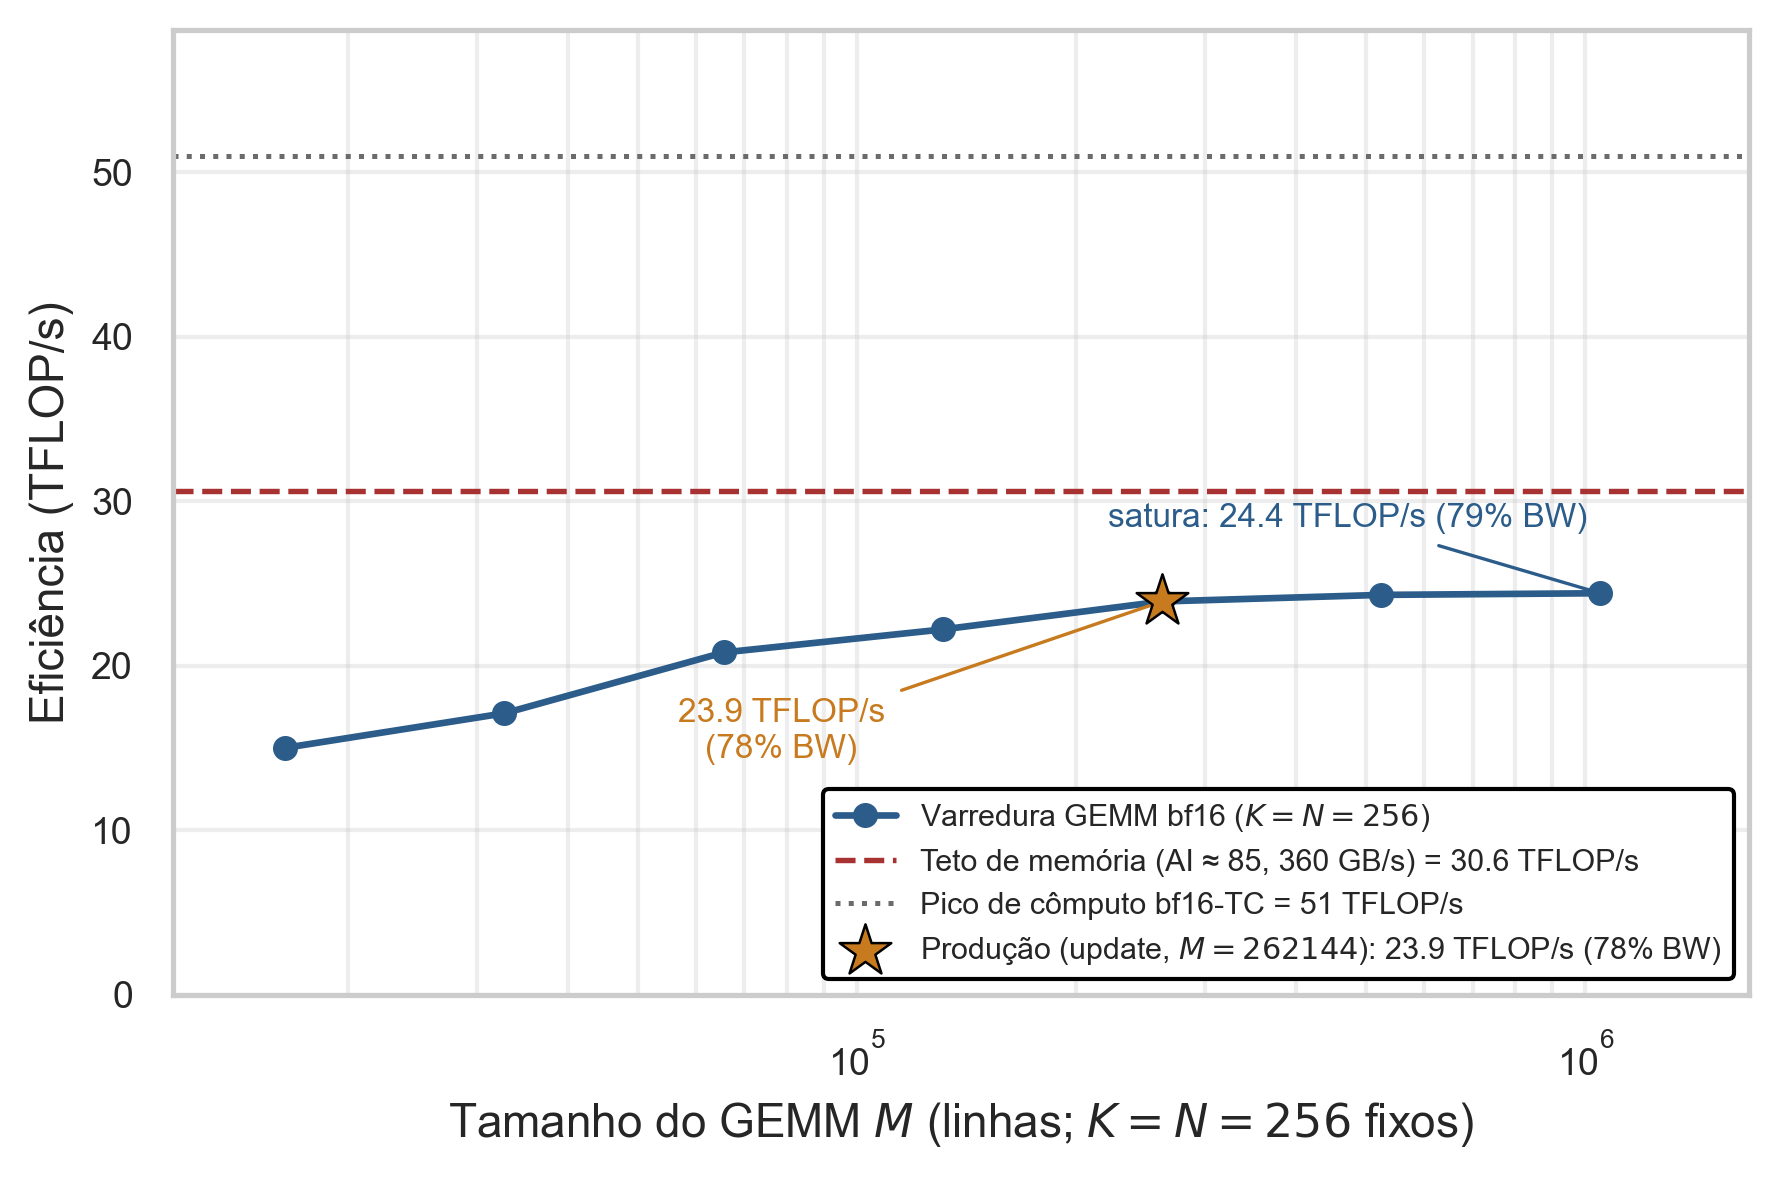
\includegraphics[width=0.7\linewidth]{roofline.png}
\caption{Varredura roofline do GEMM do update (bf16, $K{=}N{=}256$) na
RTX~3060: no tamanho de produção ($M{\approx}262\,144$) opera a $23{,}9$ TFLOP/s
($78\%$ da banda), saturando em ${\sim}24{,}4$ ($79\%$) para $M$ maiores ---
confirmando o regime memory-bound ($\mathrm{AI}{=}85 <$ ridge ${=}142$).}
\label{fig:roofline}
\end{figure}

\subsection{Pilar 2 --- Precisão mista}\label{sec:precisao}

A Tabela~\ref{tab:speedups} decompõe a contribuição de cada alavanca de
execução avaliada, com veredito honesto.

\begin{table}[ht]
\centering
\caption{Alavancas de execução: microbenchmark vs.\ efeito ponta a ponta (e2e).}
\label{tab:speedups}
\small
\begin{tabular}{lccl}
\toprule
Alavanca & Micro & E2e & Veredito\\
\midrule
bf16 autocast & $1{,}97\times$ (update) & $\mathbf{1{,}87\times}$ (992$\to$529 ms) & A alavanca real. A/B: sem degradação\\
\texttt{torch.compile} (update) & $1{,}10$--$1{,}14\times$ & $+9\%$ (6,8$\to$7,6 M SPS) & Ganho modesto, gratuito\\
Triton fundido (GELU(XW+b)) & $\mathbf{2{,}88\times}$ vs cuBLAS & $+2\%$ & Op é memory-bound; rollout é 30\% da época\\
CUDA graphs & --- & $\sim 1{,}05\times$ & Paridade (o ``1,52$\times$'' era espantalho)\\
Staleness de gradiente ($K{=}2$) & $1{,}50\times$ (update) & $1{,}35\times$ & \textbf{Revertido}: degrada o aprendizado\\
int8 (cuBLAS / Triton) & $0{,}89$--$1{,}05\times$ & --- & Morto: kernel é occupancy-bound\\
\bottomrule
\end{tabular}
\end{table}

\textbf{bf16: a alavanca real.} O bf16 é o resultado central deste pilar:
$1{,}87\times$ ponta a ponta (época de 992~ms em TF32 para 529~ms em bf16),
validado por A/B de \emph{aprendizado} com 3 sementes a partir de um
checkpoint de produção ($+200$M passos cada braço): retorno TF32 $627{,}5$
(desvio $27{,}3$) vs.\ bf16 $639{,}5$ --- diferença dentro do ruído --- e zero
NaN em 270 bilhões de passos subsequentes de produção. O roofline da
Seção~\ref{sec:throughput} explica o porquê: metade dos bytes por elemento
$\Rightarrow$ o dobro de elementos pela mesma banda. Uma ablação com
\emph{workload} fixo (precisão $\times$ compilação) confirma que o eixo de
precisão domina os ganhos, com a compilação contribuindo apenas marginalmente.

\textbf{Kernelização: paridade e espantalhos.} Pelo mesmo diagnóstico, as
alavancas que não reduzem bytes renderam pouco. CUDA graphs deram
${\sim}1{,}05\times$ contra a produção real (o $1{,}52\times$ inicial era
medido contra um baseline espantalho; Seção~\ref{sec:analise-medicao}). O
\emph{kernel} Triton fundido $\mathrm{GELU}(XW{+}b)$ é legitimamente
$2{,}88\times$ mais rápido que cuBLAS $+$ GELU separados em microbenchmark
(0,807 $\to$ 0,281~ms) --- fusão elimina uma ida e volta à HBM em uma operação
memory-bound --- mas sobreviveu à integração como apenas $+2\%$ ponta a ponta,
porque o rollout é só ${\sim}30\%$ da época; a variante multi-camada
totalmente fundida esbarrou no limite de memória compartilhada e não foi
concluída. A lição, quantificada: \emph{neste regime, o ganho veio de
precisão, não de kernelização}.

\textbf{NF4-QAT: compressão da política.} Na ponta agressiva do espectro de
precisão, a política treinada sob NF4-QAT (quantização NormalFloat-4
\cite{dettmers2023} no forward, gradiente \emph{straight-through}) converge
normalmente e produz um artefato $8\times$ menor que o fp32. Ressalva
metodológica explícita: o NF4 permaneceu \emph{sempre ligado} nos treinos
dessa linha --- não existe A/B fp32-vs-NF4 de recompensa final. Sem essa
ablação, o NF4 conta como infraestrutura funcionando, não como claim de que 4
bits bastam sem custo; a ablação é trabalho futuro.

\subsection{Pilar 3 --- Escalabilidade}\label{sec:escalabilidade}

Distinguimos duas dimensões de escala, deliberadamente: escalar o
\emph{sistema} e escalar o \emph{problema}. A primeira foi entregue; a
segunda é onde o estudo encontra sua fronteira.

\textbf{(a) Escalar o sistema.} Os dois pilares anteriores compõem: 32\,768
ambientes paralelos residentes na GPU, 7--8M passos/s sustentados, e
estabilidade numérica suficiente (zero NaN sob bf16) para campanhas
ininterruptas de dias. É isso que torna executáveis, em uma única GPU de
consumo, orçamentos de $10^{11}$--$10^{12}$ passos --- o experimento $n{=}5$
acumulou $1{,}6$ trilhão de passos. Sem essa escala de sistema, a escada de
$n$ abaixo sequer poderia ser tentada com PPO e ação discreta.

\textbf{(b) Escalar o problema: a escada de $n$.}\label{sec:reward-n}

A Tabela~\ref{tab:reward-n} consolida o resultado de controle por $n$. O teto
teórico de retorno por episódio é ${\sim}2250$ (1500 passos $\times$ 1,5).

\begin{table}[ht]
\centering
\caption{Resultado de swing-up por $n$ (linha principal, observação completa,
exceto onde indicado). \%up $=$ fração do tempo com $\cos\theta > 0{,}6$.}
\label{tab:reward-n}
\small
\begin{tabular}{llrrl}
\toprule
Config & Política & Retorno / teto & \%up & Veredito\\
\midrule
$n=1$ full-obs & MLP & 2188 / 2250 & 97\% & \textbf{Resolvido}\\
$n=1$ POMDP $(x,\dot{x})$ & LSTM & --- & \textbf{96,8\%} (245B) & \textbf{Resolvido às cegas}\\
$n=1$ POMDP $(x,\dot{x})$ & MLP & --- & ${\sim}11\%$ & Controle negativo: falha\\
$n=2$ POMDP & LSTM & --- & ${\sim}38\%$ & Em progresso\\
$n=4$ full-obs & MLP & 1031 / 2250 & n/d & Parcial / instável\\
$n=5$ full-obs & MLP & 610--624 / 2250 & n/d (${\sim}27\%$ do teto) & \textbf{Não resolvido} (1,6 T passos)\\
\bottomrule
\end{tabular}
\end{table}

\textbf{$n=1$: o PPO brilha.} Com observação completa, o swing-up é resolvido
com folga (2188 de 2250; 97\% do tempo ereto). Mais notável é a variante às
cegas: observando \emph{apenas} o carrinho, a LSTM com TBPTT stateful atinge
96,8\% ereto aos 245 bilhões de passos --- estatisticamente o mesmo teto do
agente que enxerga tudo. A memória recupera integralmente a observabilidade; o
custo da cegueira é eficiência amostral (${\sim}20$--$40\times$ mais passos),
não teto de desempenho. O controle negativo confirma o desenho: a mesma
observação parcial com MLP sem memória estaciona em ${\sim}11\%$.

\textbf{$n=5$: a fronteira.} A Figura~\ref{fig:n5curve} mostra a curva de
aprendizado. A progressão é real mas brutalmente lenta: retorno 61 aos 100
milhões de passos, 372 aos 500 milhões, platô em ${\sim}470$ por centenas de
bilhões, e \emph{warm-restarts} de LR arrancando ganhos decrescentes ---
$530 \to 612{,}6$ no primeiro ciclo (1T), sem recuperação do nível anterior no
segundo (2T, interrompido a 1,4T por reboot; retomou a ${\sim}575$). O melhor
resultado, ${\sim}610$--$624$ de 2250 (${\sim}27\%$ do teto), foi obtido com
$1{,}6$ trilhão de passos acumulados. Os episódios sobrevivem os 1500 passos
inteiros: a política aprendeu a não falhar, mas não a completar o swing-up dos
5 elos. É um platô de otimização/exploração, não de sobrevivência.

\begin{figure}[ht]
\centering
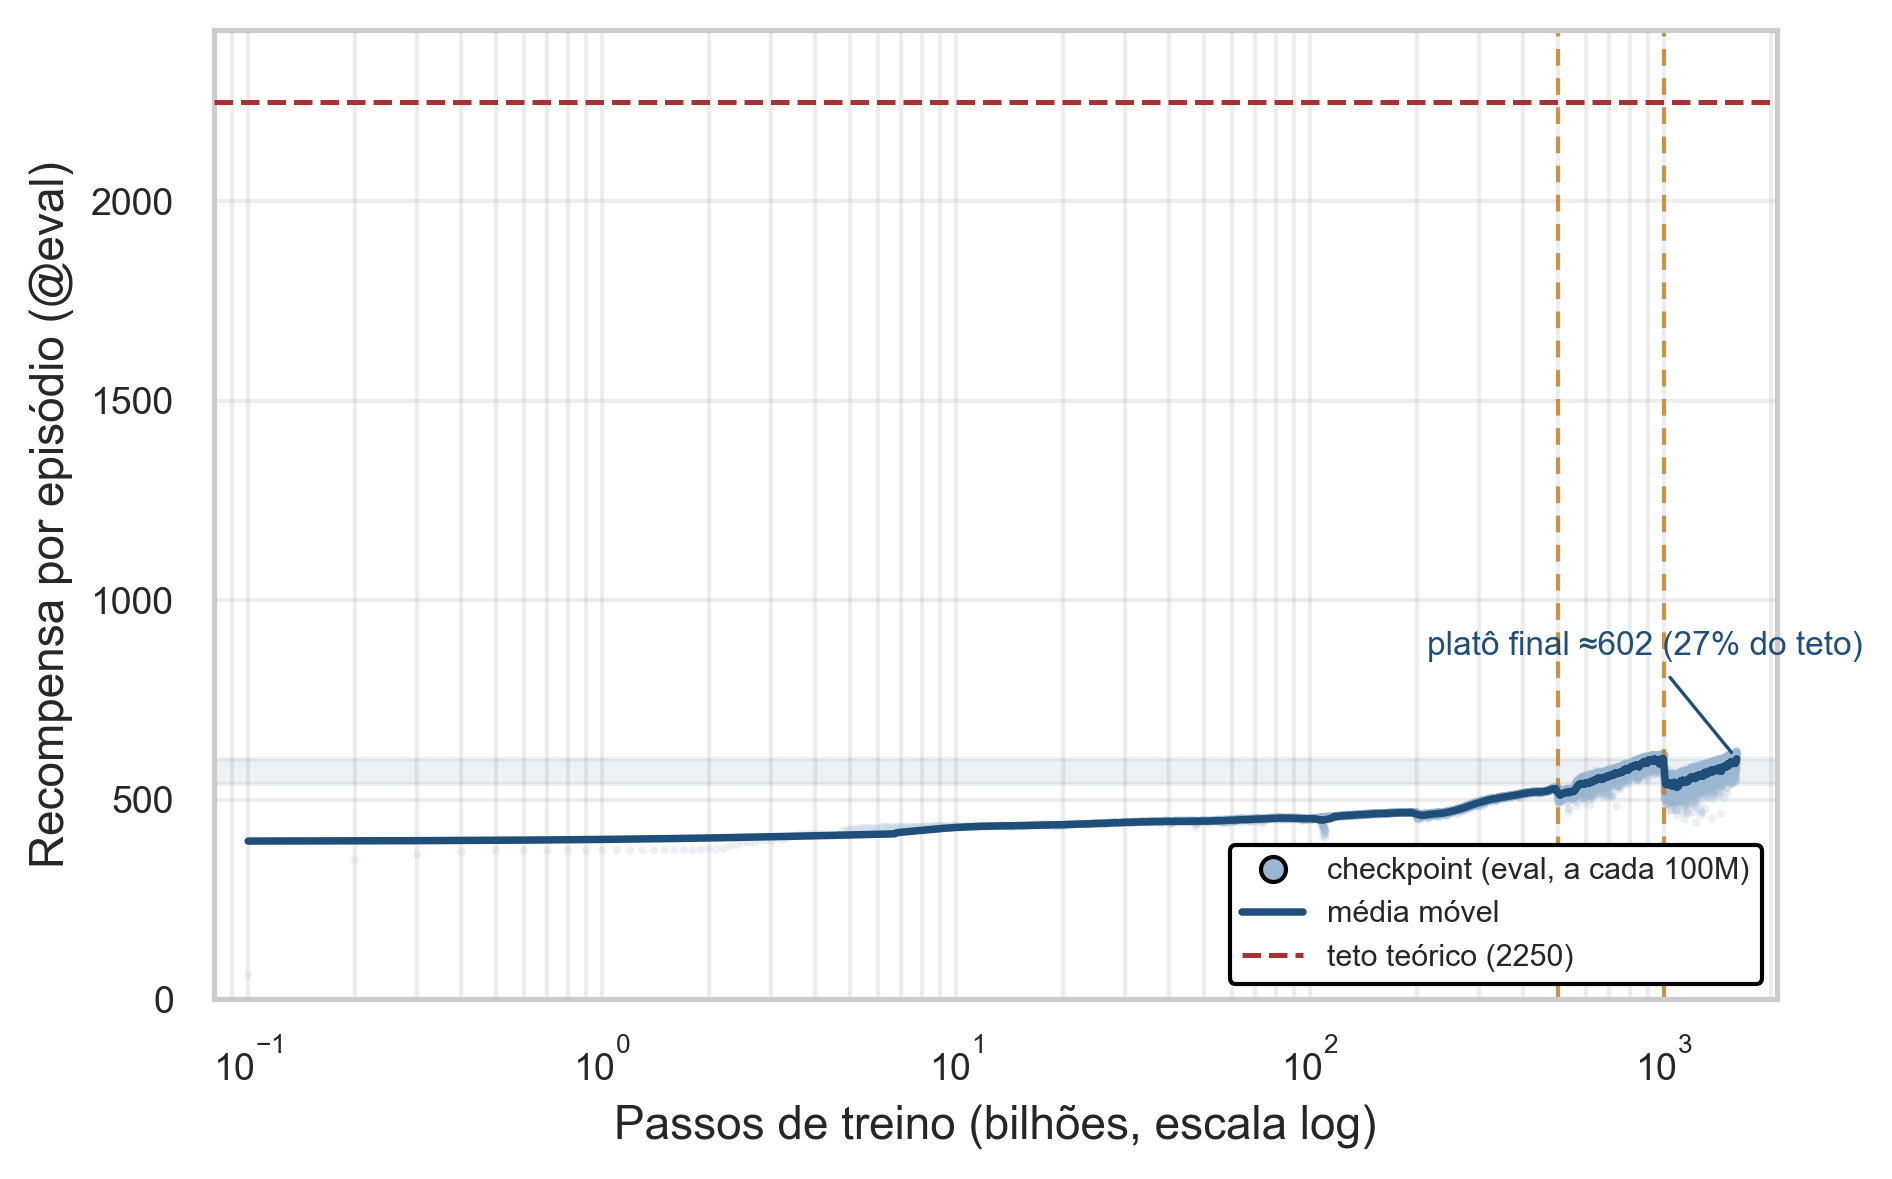
\includegraphics[width=0.7\linewidth]{n5_reward.png}
\caption{Curva de recompensa do $n{=}5$ (completa, até $1{,}6$~T passos, eixo
$x$ em escala log): salto inicial, platô longo e ganhos decrescentes por
warm-restart de LR (linhas verticais). O platô final ${\approx}602$ fica em
${\sim}27\%$ do teto teórico (2250) --- fronteira aberta.}
\label{fig:n5curve}
\end{figure}

% =========================================================================
\section{Análise}\label{sec:analise}

A análise espelha os três pilares: por que o throughput é a alavanca
(Seção~\ref{sec:analise-capacidade}), o que a precisão mista ensinou sobre
medição (Seção~\ref{sec:analise-medicao}) e o que acontece ao escalar o
problema (Seções~\ref{sec:analise-quebra} e~\ref{sec:analise-pomdp}).

\subsection{Pilar 1 --- Por que throughput é a alavanca: capacidade não é o
gargalo}\label{sec:analise-capacidade}

O argumento central se sustenta em três evidências convergentes. Primeiro, a
dimensionalidade: a observação de $n{=}5$ tem 17 números; a de $n{=}21$ teria
65. Uma MLP $2\times256$ ($\sim$140K parâmetros) é vasta para funções nesse
domínio --- e de fato o $n{=}1$ é resolvido com folga por essa rede, inclusive
na versão POMDP em que a LSTM precisa manter um filtro de estado interno.
Segundo, o modo de falha do $n{=}5$: os episódios não terminam por queda ---
a política domina a sobrevivência --- mas o retorno estaciona. Se capacidade
fosse o gargalo, veríamos subajuste também nas competências parciais; o que
vemos é uma política competente presa em uma bacia de comportamento, sintoma
de \emph{exploração} insuficiente sobre uma paisagem de recompensa com
gradiente quase nulo entre ``balançar alto'' e ``completar o swing-up de 5
elos''. Terceiro, a aritmética do orçamento: cada $1{,}87\times$ de throughput
transformou semanas de GPU em dias e viabilizou os regimes de $10^{11}$--%
$10^{12}$ passos em hardware de consumo --- foi o bf16, não qualquer mudança
algorítmica, que tornou o experimento de 1,6 trilhão de passos executável.
Nesse regime, otimizações de sistemas \emph{são} metodologia científica: elas
definem quais perguntas cabem no hardware.

\subsection{Pilar 2 --- Precisão vs.\ kernelização: lições de medição}
\label{sec:analise-medicao}

\textbf{Baseline de produção, não espantalho.}\label{sec:graph} CUDA graphs
pareceram render $1{,}52\times$ --- mas contra uma réplica com política
\emph{aleatória}, que derruba o pêndulo e gera ${\sim}42$ mil sincronizações
device$\to$host por época. Contra a produção real (política treinada, que
completa os 1500 passos e quase não sincroniza) o ganho é ${\sim}1{,}05\times$:
paridade. O mesmo condenou o Triton ($2{,}88\times$ micro, $+2\%$ real), cujo
microbenchmark comparava contra um cuBLAS artificialmente lento. Lição:
\emph{speedup contra espantalho não sobrevive à integração}.

\textbf{Throughput não é o objetivo, aprendizado é.}\label{sec:staleness}
Reusar gradientes por 2 minibatches deu $1{,}35\times$ e \emph{pareceu} inócuo
por 500M passos; sob observação sustentada (2,5B) o retorno degradou
monotonicamente ($454 \to 426$) e foi revertido. Um A/B curto pode aprovar uma
perda lenta.

\textbf{Medir o valor físico, não o proxy.} No \emph{center-farming}
(Seção~\ref{sec:pomdp-metodo}), o controle negativo (MLP cega) teve retorno
\emph{maior} que o full-obs (212 vs.\ 66) --- parado no centro, colhendo o
termo $\mathrm{center}$ com o pêndulo pendurado; só a métrica física
($\cos\theta$ do simulador) revelou o hack. E aos 245B, o agente cego reportava
\%up igual ao full-obs, mas o \emph{vídeo} revelou $4\times$ mais velocidade de
carrinho --- sensoriamento ativo do POMDP, invisível a qualquer escalar
agregado.

\subsection{Pilar 3 --- Onde o PPO quebra ao crescer $n$}
\label{sec:analise-quebra}

A degradação $n{=}1$ (97\%) $\to$ $n{=}4$ (parcial) $\to$ $n{=}5$ (27\% do
teto) tem causas identificáveis. O espaço de estados cresce ($2n+2$
dimensões), mas o fator dominante é a interação entre \textbf{subatuação e
caos}: com um único atuador para $n{+}1$ graus de liberdade, a sequência de
chaveamentos que bombeia energia \emph{coerentemente} para todos os elos é uma
agulha em um palheiro que cresce exponencialmente --- e a dinâmica caótica
pune qualquer imprecisão de fase. A recompensa densa em altura
(Eq.~\ref{eq:reward}) guia bem os primeiros elos, mas o gradiente
comportamental entre ``4 elos altos oscilando'' e ``5 elos travados no topo''
é quase invisível para exploração por perturbação local de uma política
determinística-em-média. Os warm-restarts de LR --- que escapam de bacias
locais e re-convergem --- extraíram $+15\%$, com retornos decrescentes por
ciclo, exatamente o comportamento esperado quando o problema é a paisagem de
exploração e não a otimização local. As saídas prováveis (currículo sobre $n$
ou sobre gravidade, transferência de $n{-}1 \to n$, \emph{shaping} de energia
à la \cite{astrom2000}) mudam a paisagem, não o otimizador. Em síntese:
escalar o sistema foi resolvido; escalar o problema é a pergunta de pesquisa
que o sistema agora permite formular com precisão.

\subsection{Pilar 3 --- O resultado POMDP e o mecanismo do TBPTT}
\label{sec:analise-pomdp}

O experimento às cegas quase falhou por uma razão sutil: com BPTT
reiniciando de $h{=}0$ a cada janela de 128 passos, a LSTM treinava sobre uma
trajetória de crença ``fria'' diferente da trajetória ``quente'' (acumulada
por até 1500 passos) que gerou as ações --- corrompendo a atribuição de
crédito. Com esse defeito, a recorrente empatava com o controle negativo
(${\sim}11\%$). O TBPTT stateful (janela inicializada com o estado oculto real
do rollout) destravou a curva: 25\% aos 9B, 50\% aos 40B, 96,8\% aos 245B. O
resultado final --- inferir e inverter um pêndulo que nunca se observa,
apenas pelas reações do carrinho --- é, a nosso ver, a demonstração mais
limpa do artigo de que o PPO com o orçamento certo de amostras resolve
problemas de estimação-e-controle não triviais.

\subsection{Limitações}\label{sec:limitacoes}

Com a mesma honestidade: (i) $n{=}4$ é parcial e $n{=}5$ está \emph{não
resolvido} --- 27\% do teto após 1,6T passos; throughput sozinho não venceu a
paisagem de exploração para $n \geq 4$. (ii) A linha principal em CUDA ainda
carrega o termo $\mathrm{center}$ farmável na recompensa
(Eq.~\ref{eq:reward}); a correção existe apenas na variante POMDP, e os
retornos de $n \geq 4$ devem ser lidos com essa ressalva. (iii) As métricas
\%up de $n{=}4$ e $n{=}5$ não foram logadas --- reportamos retorno/teto, um
proxy que a Seção~\ref{sec:analise-medicao} nos ensinou a desconfiar.
(iv) O NF4-QAT não tem A/B de qualidade. (v) Os resultados de throughput são
de uma única GPU (RTX 3060); as conclusões roofline devem transferir para
outras arquiteturas memory-bound, mas não foram verificadas nelas.

% =========================================================================
\section{Conclusões}\label{sec:conclusao}

Este trabalho tratou o swing-up do pêndulo-$N$ subatuado como um problema de
\emph{orçamento de amostras}, estudado nos três eixos do título. Em
\textbf{throughput}, um ambiente pêndulo-$N$ genérico e 100\% residente em GPU
sustenta 7--8M passos/s ponta a ponta em uma RTX~3060 --- a alavanca que
financia a exploração, já que a capacidade da rede não é o gargalo. Em
\textbf{precisão mista}, o resultado central é que, num laço memory-bound, a
\emph{precisão} (bf16, $1{,}87\times$ sem degradar o aprendizado; NF4-QAT,
$8\times$) vale mais que a kernelização (que rendeu paridade) --- e a própria
metodologia de medição (baseline de produção, A/B multi-semente sustentado) é
contribuição. Em \textbf{escalabilidade}, o sistema escala (trilhões de passos
em GPU de consumo) e é isso que permite \emph{tentar} escalar o problema: o PPO
resolve $n{=}1$ com folga, inclusive às cegas por LSTM (96,8\% ereto observando
só o carrinho), fica parcial em $n{=}4$ e para em $n{=}5$ (27\% do teto).
Escalar $n$ permanece, explicitamente, fronteira aberta.

Trabalhos futuros, em ordem de prioridade: (i) completar a ablação NF4
(A/B fp32 vs.\ NF4 de recompensa final); (ii) atacar $n \geq 5$ mudando a
paisagem de exploração --- currículo sobre $n$ e sobre gravidade,
transferência $n{-}1 \to n$ e shaping de energia \cite{astrom2000} ---
mantendo o orçamento que o throughput viabiliza; (iii) vieses estruturais para
generalizar entre $n$ (codificador compartilhado por elo, 1D-conv ou
message-passing sobre a cadeia), pré-requisito para (iv) subir a escada até
$n{=}21$ e mapear como a dificuldade escala com o número de elos; e (v) concluir
o $n{=}2$ às cegas, hoje em ${\sim}38\%$ e em progresso.

% =========================================================================
\begin{thebibliography}{99}
\setlength{\itemsep}{0pt}
\setlength{\parskip}{0pt}

\bibitem[Åström e Furuta 2000]{astrom2000}
Åström, K.~J. e Furuta, K. (2000).
Swinging up a pendulum by energy control.
\emph{Automatica}, 36(2):287--295.

\bibitem[Boubaker 2013]{boubaker2013}
Boubaker, O. (2013).
The inverted pendulum benchmark in nonlinear control theory: a survey.
\emph{International Journal of Advanced Robotic Systems}, 10(5):233.

\bibitem[Dettmers et al. 2023]{dettmers2023}
Dettmers, T., Pagnoni, A., Holtzman, A., e Zettlemoyer, L. (2023).
QLoRA: Efficient finetuning of quantized LLMs.
Em \emph{Advances in Neural Information Processing Systems (NeurIPS)}.

\bibitem[Freeman et al. 2021]{freeman2021}
Freeman, C.~D., Frey, E., Raichuk, A., Girgin, S., Mordatch, I., e Bachem, O.
(2021).
Brax --- a differentiable physics engine for large scale rigid body
simulation.
Em \emph{NeurIPS Datasets and Benchmarks Track}.

\bibitem[Makoviychuk et al. 2021]{makoviychuk2021}
Makoviychuk, V., Wawrzyniak, L., Guo, Y., Lu, M., Storey, K., Macklin, M.,
Hoeller, D., Rudin, N., Allshire, A., Handa, A., e State, G. (2021).
Isaac Gym: High performance GPU-based physics simulation for robot learning.
Em \emph{NeurIPS Datasets and Benchmarks Track}.

\bibitem[Micikevicius et al. 2018]{micikevicius2018}
Micikevicius, P., Narang, S., Alben, J., Diamos, G., Elsen, E., García, D.,
Ginsburg, B., Houston, M., Kuchaiev, O., Venkatesh, G., e Wu, H. (2018).
Mixed precision training.
Em \emph{International Conference on Learning Representations (ICLR)}.

\bibitem[Petrenko et al. 2020]{petrenko2020}
Petrenko, A., Huang, Z., Kumar, T., Sukhatme, G., e Koltun, V. (2020).
Sample Factory: Egocentric 3D control from pixels at 100000 FPS with
asynchronous reinforcement learning.
Em \emph{International Conference on Machine Learning (ICML)}.

\bibitem[Schulman et al. 2016]{schulman2016}
Schulman, J., Moritz, P., Levine, S., Jordan, M., e Abbeel, P. (2016).
High-dimensional continuous control using generalized advantage estimation.
Em \emph{International Conference on Learning Representations (ICLR)}.

\bibitem[Schulman et al. 2017]{schulman2017}
Schulman, J., Wolski, F., Dhariwal, P., Radford, A., e Klimov, O. (2017).
Proximal policy optimization algorithms.
\emph{arXiv preprint arXiv:1707.06347}.

\bibitem[Shacklett et al. 2023]{shacklett2023}
Shacklett, B., Rosenzweig, L.~G., Xie, Z., Sarukkai, B., e Fatahalian, K.
(2023).
An extensible, data-oriented architecture for high-performance, many-world
simulation.
\emph{ACM Transactions on Graphics}, 42(4).

\bibitem[Spong 1995]{spong1995}
Spong, M.~W. (1995).
The swing up control problem for the Acrobot.
\emph{IEEE Control Systems Magazine}, 15(1):49--55.

\bibitem[Suárez 2024]{suarez2024}
Suárez, J. (2024).
PufferLib: Making reinforcement learning libraries and environments play
nice.
\emph{arXiv preprint arXiv:2406.12905}.

\bibitem[Weng et al. 2022]{weng2022}
Weng, J., Lin, M., Huang, S., Liu, B., Makoviichuk, D., Makoviychuk, V., Liu,
Z., Song, Y., Luo, T., Jiang, Y., Xu, Z., e Yan, S. (2022).
EnvPool: A highly parallel reinforcement learning environment execution
engine.
Em \emph{Advances in Neural Information Processing Systems (NeurIPS)}.

\end{thebibliography}

\end{document}
